\documentclass[12pt]{article}
\usepackage[margin=.75in]{geometry}
\usepackage{listings}
\usepackage{amsmath}
\usepackage{bbm}
\usepackage{amsfonts}
\usepackage{multirow}
\usepackage{makecell}
\usepackage{arydshln}
\usepackage{titlesec}
\usepackage{tikz}
\usepackage{tikz-3dplot}
\usetikzlibrary{calc}
\usepackage{float}

\pagenumbering{gobble}

\begin{document}
\setlength{\parindent}{0pt}
\titlespacing\subsection{0pt}{4pt plus 2pt minus 2pt}{2pt plus 2pt minus 2pt}

\textbf{Weeks of 6/23 + 6/30}

Kit Levy

\begin{center}
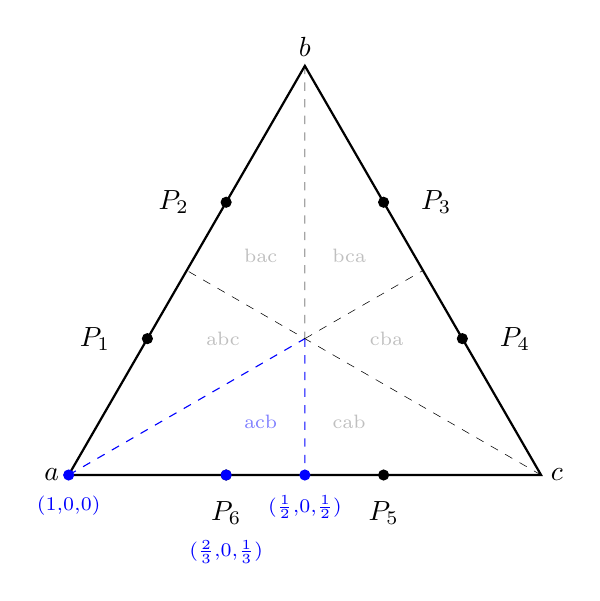
\begin{tikzpicture}[scale=6]

\coordinate (A) at (0,0);
\coordinate (B) at (0.5,{sqrt(3)/2});
\coordinate (C) at (1,0);

\draw[thick] (A) -- (B) -- (C) -- cycle;
\node[left] at (A) {\( a \)};
\node[above] at (B) {\( b \)};
\node[right] at (C) {\( c \)};

%barycentric to Cartesian macro
\newcommand{\barycentric}[3]{%
  ($#1*(A) + #2*(B) + #3*(C)$)
}

\filldraw[black] \barycentric{2/3}{1/3}{0} circle (0.3pt) node[left=10pt] {\(P_1\)};
\filldraw[black] \barycentric{1/3}{2/3}{0} circle (0.3pt) node[left=10pt] {\(P_2\)};
\filldraw[black] \barycentric{0}{2/3}{1/3} circle (0.3pt) node[right=10pt] {\(P_3\)};
\filldraw[black] \barycentric{0}{1/3}{2/3} circle (0.3pt) node[right=10pt] {\(P_4\)};
\filldraw[black] \barycentric{1/3}{0}{2/3} circle (0.3pt) node[below=6pt] {\(P_5\)};
\filldraw[black] \barycentric{2/3}{0}{1/3} circle (0.3pt) node[below=6pt] {\(P_6\)};

\filldraw[blue] \barycentric{1}{0}{0} circle (0.3pt) node[below=4pt] {\(\scriptstyle(1,0,0)\)};
\filldraw[blue] \barycentric{2/3}{0}{1/3} circle (0.3pt) node[below=20pt] {\( \scriptstyle(\frac{2}{3},0,\frac{1}{3})\)};
\filldraw[blue] \barycentric{1/2}{0}{1/2} circle (0.3pt) node[below=4pt] {\( \scriptstyle(\frac{1}{2},0,\frac{1}{2})\)};

\draw[dashed, blue, thin] \barycentric{1}{0}{0} -- \barycentric{1/3}{1/3}{1/3};
\draw[dashed, black, very thin] \barycentric{1/3}{1/3}{1/3} -- \barycentric{0}{1/2}{1/2};
\draw[dashed, black, very thin] \barycentric{0}{1}{0} -- \barycentric{1/3}{1/3}{1/3};
\draw[dashed, blue, thin] \barycentric{1/3}{1/3}{1/3} -- \barycentric{1/2}{0}{1/2};
\draw[dashed, black, very thin] \barycentric{0}{0}{1} -- \barycentric{1/2}{1/2}{0};

%\coordinate (Z) at \barycentric{1/3}{1/3}{1/3};
\node[left=20pt][opacity=0.5] at \barycentric{1/3}{1/3}{1/3} {\scriptsize \color{gray} abc};
\node[right=20pt][opacity=0.5] at \barycentric{1/3}{1/3}{1/3} {\scriptsize \color{gray} cba};
\node[left=16pt, above=24pt][opacity=0.5] at \barycentric{1/3}{1/3}{1/3} {\scriptsize \color{gray} bac};
\node[right=16pt, above=24pt][opacity=0.5] at \barycentric{1/3}{1/3}{1/3} {\scriptsize \color{gray} bca};
\node[right=16pt, below=24pt][opacity=0.5] at \barycentric{1/3}{1/3}{1/3} {\scriptsize \color{gray} cab};
\node[left=16pt, below=24pt][opacity=0.5] at \barycentric{1/3}{1/3}{1/3} {\scriptsize \color{blue} acb};

\end{tikzpicture}
\end{center}

\subsection*{\normalsize Threshold $\alpha$ values for each change in preferences:}
\renewcommand{\arraystretch}{1.3}

\begin{table}[h]
\centering
%\caption{Threshold $\alpha$ values for each change in preferences}
\resizebox{\textwidth}{!}{%
\begin{tabular}{l@{\hskip 4pt}|c@{\hskip 4pt}|c@{\hskip 4pt}:c@{\hskip 4pt}|c@{\hskip 4pt}:c@{\hskip 4pt}:c@{\hskip 4pt}:c@{\hskip 4pt}:c@{\hskip 4pt}|c@{\hskip 4pt}:c@{\hskip 4pt}|c@{\hskip 4pt}c}

 &
  \makecell{\footnotesize \textbf{P1} \\ \textbf{$\rightarrow$ acb}} &
  \makecell{\footnotesize P2 \\ $\rightarrow$ abc} &
  \makecell{\footnotesize \textbf{P2} \\ \textbf{$\rightarrow$ acb}} &
  \makecell{\footnotesize P3 \\ $\rightarrow$ bac} &
  \makecell{\footnotesize P3 \\ $\rightarrow$ abc} &
  \makecell{\footnotesize P3 \\ $\rightarrow$ cba} &
  \makecell{\footnotesize P3 \\ $\rightarrow$ cab} &
  \makecell{\footnotesize \textbf{P3} \\ \textbf{$\rightarrow$ acb}} &
  \makecell{\footnotesize P4 \\ $\rightarrow$ cab} &
  \makecell{\footnotesize \textbf{P4} \\ \textbf{$\rightarrow$ acb}} &
  \makecell{\footnotesize \textbf{P5} \\ \textbf{$\rightarrow$ acb}} \\
\hline
$(1,0,0)$ &
  1 &
  $\frac{1}{4}$ &
  1 &
  $\frac{1}{4}$ &
  $\frac{2}{5}$ &
  - &
  - &
  1 &
  $\frac{1}{4}$ &
  $\frac{2}{5}$ &
  $\frac{1}{4}$ \\
$(\frac{2}{3},0,\frac{1}{3})$ &
  $\frac{1}{2}$ &
  $\frac{1}{3}$ &
  $\frac{2}{3}$ &
  - &
  - &
  - &
  - &
  $\frac{1}{2}$ &
  $\frac{1}{3}$ &
  $\frac{2}{3}$ &
  $\frac{1}{2}$ \\
$(\frac{1}{2},0,\frac{1}{2})$ &
  $\frac{2}{5}$ &
  $\frac{2}{5}$ &
  $\frac{4}{7}$ &
  - &
  - &
  $\frac{2}{5}$ &
  $\frac{4}{7}$ &
  1 &
  $\frac{2}{5}$ &
  1 &
  1
\end{tabular}%
}
\end{table}

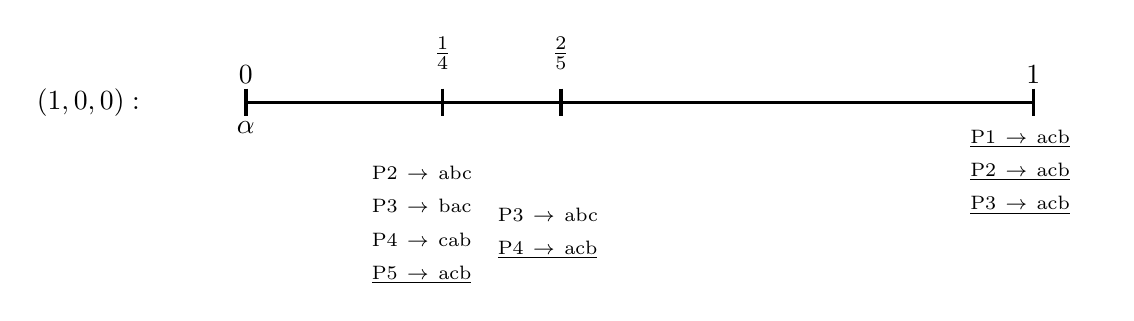
\begin{tikzpicture}[]
        \node[] at (0,0) {$(1,0,0):$};
        
        \draw[very thick] (2cm, 0cm) node[above=1mm] {0} node[below=1mm] {$\alpha$}
              --
              (12cm, 0cm) node[above=1mm] {1};

        \draw[very thick] (2 cm,5pt) -- (2 cm,-5pt);
        \draw[very thick] (12 cm,5pt) -- (12 cm,-5pt) node[text width = 1.6cm, below=1pt]{\scriptsize \underline{P1 $\rightarrow$ acb} \underline{P2 $\rightarrow$ acb} \underline{P3 $\rightarrow$ acb}};

        \draw[very thick] (4.5 cm,5pt) node[above=1mm]{$\frac{1}{4}$} -- (4.5 cm,-5pt) node[text width = 1.8cm, below=1pt]{\scriptsize \vskip 6pt P2 $\rightarrow$ abc P3 $\rightarrow$ bac P4 $\rightarrow$ cab \underline{P5 $\rightarrow$ acb}};

        \draw[very thick] (6 cm,5pt) node[above=1mm]{$\frac{2}{5}$} -- (6 cm,-5pt) node[text width = 1.6cm, below=1pt]{\scriptsize \vskip 21pt P3 $\rightarrow$ abc \underline{P4 $\rightarrow$ acb}};
            
\end{tikzpicture}

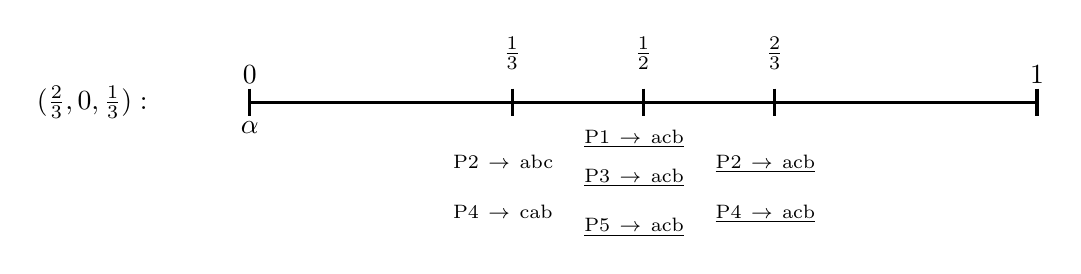
\begin{tikzpicture}[]
        \node[] at (0,0) {$(\frac{2}{3},0,\frac{1}{3}):$};
        
         \draw[very thick] (2cm, 0cm) node[above=1mm] {0} node[below=1mm] {$\alpha$}
              --
              (12cm, 0cm) node[above=1mm] {1};

        \draw[very thick] (2 cm,5pt) -- (2 cm,-5pt);
        \draw[very thick] (12 cm,5pt) -- (12 cm,-5pt);

        \draw[very thick] (5.333 cm,5pt) node[above=1mm]{$\frac{1}{3}$} -- (5.333 cm,-5pt) node[text width = 1.5cm, below=1pt]{\scriptsize \vskip 6pt P2 $\rightarrow$ abc \vskip 6pt P4 $\rightarrow$ cab};

        \draw[very thick] (7 cm,5pt) node[above=1mm]{$\frac{1}{2}$} -- (7 cm,-5pt) node[text width = 1.5cm, below=1pt]{\scriptsize \underline{P1 $\rightarrow$ acb} \vskip 6pt \underline{P3 $\rightarrow$ acb} \vskip 6pt \underline{P5 $\rightarrow$ acb}};

        \draw[very thick] (8.667 cm,5pt) node[above=1mm]{$\frac{2}{3}$} -- (8.667 cm,-5pt) node[text width = 1.5cm, below=1pt]{\scriptsize \vskip 6pt \underline{P2 $\rightarrow$ acb} \vskip 6pt \underline{P4 $\rightarrow$ acb} };
            
\end{tikzpicture}

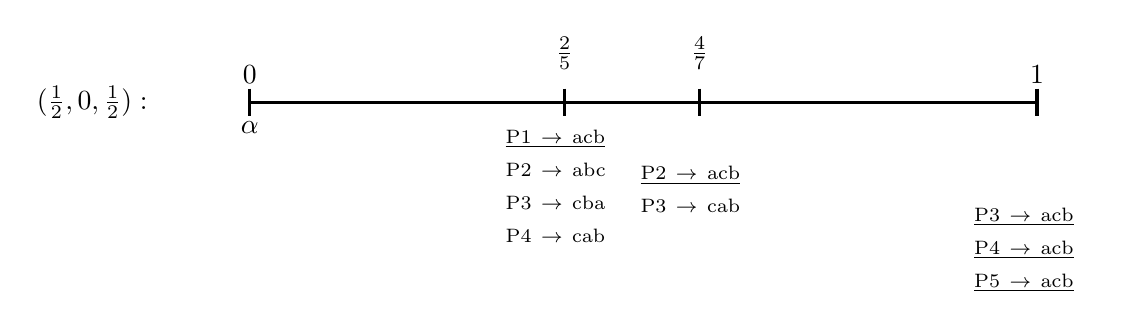
\begin{tikzpicture}[]
        \node[] at (0,0) {$(\frac{1}{2},0,\frac{1}{2}):$};
        
         \draw[very thick] (2cm, 0cm) node[above=1mm] {0} node[below=1mm] {$\alpha$}
              --
              (12cm, 0cm) node[above=1mm] {1};

        \draw[very thick] (2 cm,5pt) -- (2 cm,-5pt);
        \draw[very thick] (12 cm,5pt) -- (12 cm,-5pt) node[text width = 1.6cm, below=1pt]{\scriptsize \vskip 21pt \underline{P3 $\rightarrow$ acb} \underline{P4 $\rightarrow$ acb} \underline{P5 $\rightarrow$ acb}};

        \draw[very thick] (6 cm,5pt) node[above=1mm]{$\frac{2}{5}$} -- (6 cm,-5pt) node[text width = 1.5cm, below=1pt]{\scriptsize \underline{P1 $\rightarrow$ acb} P2 $\rightarrow$ abc P3 $\rightarrow$ cba P4 $\rightarrow$ cab};

        \draw[very thick] (7.714 cm,5pt) node[above=1mm]{$\frac{4}{7}$} -- (7.714 cm,-5pt) node[text width = 1.5cm, below=1pt]{\scriptsize \vskip 6pt \underline{P2 $\rightarrow$ acb} P3 $\rightarrow$ cab};
            
\end{tikzpicture}

\subsection*{\normalsize Voters who rank $a > c > b$ as a function of $\alpha$:}

\underline{$w = (1,0,0)$:} $P_{acb} = P6 + \mathbbm{1}\{\alpha = 1\}(P1 + P2 + P3) + \mathbbm{1}\{\alpha \geq \frac{2}{5}\}P4 + \mathbbm{1}\{\alpha \geq \frac{1}{4}\}P5$

\underline{$w = (\frac{2}{3},0,\frac{1}{3})$:} $P_{acb} = P6 + \mathbbm{1}\{\alpha \geq \frac{1}{2}\}(P1 + P3 + P5) + \mathbbm{1}\{\alpha \geq \frac{2}{3}\}(P2 + P4)$

\underline{$w = (\frac{1}{2}, 0, \frac{1}{2})$:} $P_{acb} = P6 + \mathbbm{1}\{\alpha \geq \frac{2}{5}\}P1 + \mathbbm{1}\{\alpha \geq \frac{4}{7}\}P2 + \mathbbm{1}\{\alpha = 1\}(P3 + P4 + P5)$

\vskip \baselineskip
\subsection*{\normalsize Choosing $w$ to achieve $a > c > b$ based on known $\alpha$ (ignoring effects of IA):}

\begin{table}[H]
\centering
\begin{tabular}{l|l}
\textbf{$\alpha$}                       & \textbf{Best $w$ (highest $P_{acb}$)}                                  \\ \hline
$\alpha < \frac{1}{4}$                  & None                                                                    \\ \hline
$\frac{1}{4} \leq \alpha < \frac{2}{5}$ & $(1,0,0)$                                                               \\ \hline
$\frac{2}{5} \leq \alpha < \frac{1}{2}$ & $(1,0,0)$ if $P4 + P5 > P1$                                             \\
                                        & $(\frac{1}{2},0,\frac{1}{2})$ if $P1 > P4 + P5$                         \\ \hline
$\frac{1}{2} \leq \alpha < \frac{4}{7}$ & $(1,0,0)$ if $P4 > P1 + P3$                                             \\
                                        & $(\frac{2}{3},0,\frac{1}{3})$ if $P1 + P3 > P4$                         \\ \hline
$\frac{4}{7} \leq \alpha < \frac{2}{3}$ & $(1,0,0)$ if $P4 > P1 + P3$ and $P4 + P5 > P1 + P2$                     \\
                                        & $(\frac{2}{3},0,\frac{1}{3})$ if $P1 + P3 > P4$ and $P3 + P5 > P2$      \\
                                        & $(\frac{1}{2},0,\frac{1}{2})$ if $P1 + P2 > P4 + P5$ and $P2 > P3 + P5$ \\ \hline
$\frac{2}{3} \leq \alpha < 1$           & $(\frac{2}{3},0,\frac{1}{3})$                                           \\ \hline
$\alpha = 1$                            & Any                                                               
\end{tabular}
\end{table}

\subsection*{\normalsize Movement into and out of IA according to $\alpha$ and $w$:}

\begin{table}[H]
\centering
\begin{tabular}{l|l|l|l}
Voter               & $w$                           & $\alpha$ for which voter is in IA       & ``Time'' spent in IA \\ \hline
P1                  & Any                           & None                                    & 0                  \\ \hline
\multirow{3}{*}{P2} & $(1,0,0)$                     & $\frac{1}{4} \leq \alpha < 1$           & $\frac{3}{4}$      \\
                    & $(\frac{2}{3},0,\frac{1}{3})$ & $\frac{1}{3} \leq \alpha < \frac{2}{3}$ & $\frac{1}{3}$      \\
 & $(\frac{1}{2},0,\frac{1}{2})$ & $\frac{2}{5} \leq \alpha < \frac{4}{7}$ & $\frac{6}{35}$ \\ \hline
\multirow{3}{*}{P3} & $(1,0,0)$                     & $\frac{1}{4} \leq \alpha < 1$           & $\frac{3}{4}$      \\
                    & $(\frac{2}{3},0,\frac{1}{3})$ & None                                    & 0                  \\
                    & $(\frac{1}{2},0,\frac{1}{2})$ & $\frac{2}{5} \leq \alpha < 1$           & $\frac{3}{5}$      \\ \hline
\multirow{3}{*}{P4} & $(1,0,0)$                     & $\frac{1}{4} \leq \alpha < \frac{2}{5}$ & $\frac{3}{20}$     \\
                    & $(\frac{2}{3},0,\frac{1}{3})$ & $\frac{1}{3} \leq \alpha < \frac{2}{3}$ & $\frac{1}{3}$      \\
                    & $(\frac{1}{2},0,\frac{1}{2})$ & $\frac{2}{5} \leq \alpha < 1$           & $\frac{3}{5}$      \\ \hline
P5                  & Any                           & None                                    & 0                 
\end{tabular}
\end{table}

\vskip \baselineskip
\subsection*{\normalsize Plurality votes as a function of $\alpha$:}

\subsubsection*{$w = (1, 0, 0)$:}

$\operatorname{plurality}_a(\alpha) = P6 + P1 + \mathbbm{1}\{\alpha \geq \frac{1}{4}\}(P2 + P5) + \mathbbm{1}\{\alpha \geq \frac{2}{5}\}(P3 + P4)$

$\operatorname{plurality}_b(\alpha) = \mathbbm{1}\{\alpha < \frac{1}{4}\}P2 + \mathbbm{1}\{\alpha < \frac{2}{5}\}P3$

$\operatorname{plurality}_c(\alpha) = \mathbbm{1}\{\alpha < \frac{2}{5}\}P4 + \mathbbm{1}\{\alpha < \frac{1}{4}\}P5$

\subsubsection*{$w = (\frac{2}{3},0,\frac{1}{3})$:}

$\operatorname{plurality}_a(\alpha) = P1 + P6 + \mathbbm{1}\{\alpha \geq \frac{1}{3}\}P2 + \mathbbm{1}\{\alpha \geq \frac{1}{2}\}(P3 + P5) + \mathbbm{1}\{\alpha \geq \frac{2}{3}\}P4$

$\operatorname{plurality}_b(\alpha) = \mathbbm{1}\{\alpha < \frac{1}{3}\}P2 + \mathbbm{1}\{\alpha < \frac{1}{2}\}P3$

$\operatorname{plurality}_c(\alpha) = \mathbbm{1}\{\alpha < \frac{2}{3}\}P4 + \mathbbm{1}\{\alpha < \frac{1}{2}\}P5$

\subsubsection*{$w = (\frac{1}{2}, 0, \frac{1}{2})$:}

$\operatorname{plurality}_a(\alpha) = P1 + P6 + \mathbbm{1}\{\alpha \geq \frac{2}{5}\}P2 + \mathbbm{1}\{\alpha = 1\}(P3 + P4 + P5)$

$\operatorname{plurality}_b(\alpha) = \mathbbm{1}\{\alpha < \frac{2}{5}\}(P2 + P3)$

$\operatorname{plurality}_c(\alpha) = \mathbbm{1}\{\frac{2}{5} \leq \alpha < 1\}P3 + \mathbbm{1}\{\alpha < 1\}(P4 + P5)$

\vskip \baselineskip
\subsection*{\normalsize Borda votes as a function of $\alpha$:}

\subsubsection*{$w = (1, 0, 0)$:}

$\operatorname{borda}_a(\alpha) = 2P1 + P2 + P5 + 2P6 + \mathbbm{1}\{\alpha \geq \frac{1}{4}\}(P2 + P3 + P4 + P5) + \mathbbm{1}\{\alpha \geq \frac{2}{5}\}(P3 + P4)$

$\operatorname{borda}_b(\alpha) = \mathbbm{1}\{\alpha < 1\}(P1 + P2 + P3) + \mathbbm{1}\{\alpha < \frac{1}{4}\}(P2 + P4) +  \mathbbm{1}\{\alpha < \frac{2}{5}\}P3$

$\operatorname{borda}_c(\alpha) = P4 + P5 + \mathbbm{1}\{\alpha = 1\}(P1 + P2 + P3) + \mathbbm{1}\{\alpha < \frac{1}{4}\}(P3 + P5) + \mathbbm{1}\{\alpha < \frac{2}{5}\}P4$

\subsubsection*{$w = (\frac{2}{3},0,\frac{1}{3})$:}

$\operatorname{borda}_a(\alpha) = 2P1 + P2 + P5 + 2P6 + \mathbbm{1}\{\alpha \geq \frac{1}{3}\}(P2 + P4) + \mathbbm{1}\{\alpha \geq \frac{1}{2}\}(2P3 + P5) + \mathbbm{1}\{\alpha \geq \frac{2}{3}\}P4$

$\operatorname{borda}_b(\alpha) = \mathbbm{1}\{\alpha < \frac{1}{2}\}(P1 + 2P3) + \mathbbm{1}\{\alpha < \frac{1}{3}\}(P2 + P4) + \mathbbm{1}\{\alpha < \frac{2}{3}\}P2$

$\operatorname{borda}_c(\alpha) = P3 + P4 + P5 + \mathbbm{1}\{\alpha \geq \frac{1}{2}\}P1 + \mathbbm{1}\{\alpha \geq \frac{2}{3}\}P2 + \mathbbm{1}\{\alpha < \frac{2}{3}\}P4 + \mathbbm{1}\{\alpha < \frac{1}{2}\}P5$

\subsubsection*{$w = (\frac{1}{2}, 0, \frac{1}{2})$:}

$\operatorname{borda}_a(\alpha) = 2P1 + P2 + P5 + 2P6 + \mathbbm{1}\{\alpha \geq \frac{2}{5}\}(P2 + P4) + \mathbbm{1}\{\alpha \geq \frac{4}{7}\}P3 + \mathbbm{1}\{\alpha = 1\}(P3 + P4 + P5)$

$\operatorname{borda}_b(\alpha) = \mathbbm{1}\{\alpha < \frac{2}{5}\}(P1 + P2 + P3 + P4) + \mathbbm{1}\{\alpha < \frac{4}{7}\}(P2 + P3)$

$\operatorname{borda}_c(\alpha) = P3 + P4 + P5 + \mathbbm{1}\{\alpha \geq \frac{2}{5}\}P1 + \mathbbm{1}\{\alpha \geq \frac{4}{7}\}P2 + \mathbbm{1}\{\frac{2}{5} \leq \alpha < 1\}P3 + \mathbbm{1}\{\alpha < 1\}(P4 + P5)$

\subsection*{\normalsize Forced full preferences problem (IRV):}

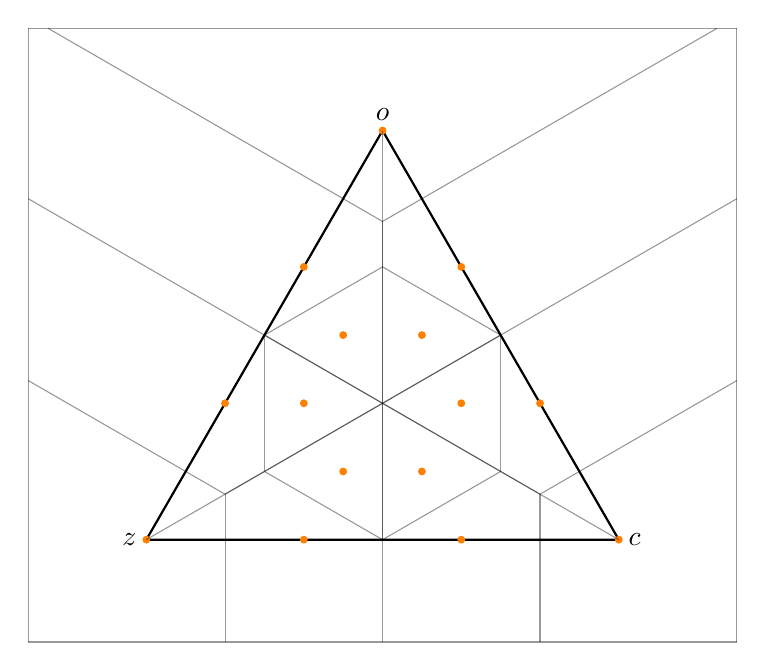
\begin{tikzpicture}[scale=6]

\coordinate (A) at (0,0);
\coordinate (B) at (0.5,{sqrt(3)/2});
\coordinate (C) at (1,0);
\draw[thick] (A) -- (B) -- (C) -- cycle;
\node[left] at (A) {\( z \)};
\node[above] at (B) {\( o \)};
\node[right] at (C) {\( c \)};

%barycentric to cartesian macro
\newcommand{\barycentric}[3]{($#1*(A) + #2*(B) + #3*(C)$)}

%Voronoi points
\foreach \point in {
  (0,0),
  (0.5,{sqrt(3)/2}),
  (1,0),
  (1/6,{1/(2*sqrt(3))}),
  (1/3,{1/sqrt(3)}),
  (1/3,0),
  (2/3,0),
  (2/3,{1/sqrt(3)}),
  (5/6,{1/(2*sqrt(3))}),
  (1/3,{1/(2*sqrt(3))}),
  (5/12,{1/(4*sqrt(3))}),
  (5/12,{sqrt(3)/4}),
  (7/12,{1/(4*sqrt(3))}),
  (7/12,{sqrt(3)/4}),
  (2/3,{1/(2*sqrt(3))})
} {
  \filldraw[orange] \point circle (0.2pt);
}


\draw[thin,opacity=0.4]\barycentric{1}{0}{0} -- \barycentric{0}{1/2}{1/2};
\draw[thin,opacity=0.4]\barycentric{0}{1}{0} -- \barycentric{1/2}{0}{1/2};
\draw[thin,opacity=0.4]\barycentric{0}{0}{1} -- \barycentric{1/2}{1/2}{0};

%exported from Mathematica
\draw[thin, opacity=0.4] (-0.20833333333333126, 1.0825317547305482) -- (0.5, 0.6735753140545634);
\draw[thin, opacity=0.4] (0.5, 0.6735753140545634) -- (1.2083333333333328, 1.0825317547305482);
\draw[thin, opacity=0.4] (1.2083333333333328, 1.0825317547305482) -- (-0.20833333333333126, 1.0825317547305482);
\draw[thin, opacity=0.4] (1.25, -0.21650635094610965) -- (1.25, 0.33678765702728164);
\draw[thin, opacity=0.4] (1.25, 0.33678765702728164) -- (0.8333333333333335, 0.09622504486493764);
\draw[thin, opacity=0.4] (0.8333333333333335, 0.09622504486493764) -- (0.8333333333333335, -0.21650635094610965);
\draw[thin, opacity=0.4] (0.8333333333333335, -0.21650635094610965) -- (1.25, -0.21650635094610965);
\draw[thin, opacity=0.4] (0.5, 0.2886751345948129) -- (0.5, 1.0816665110907547e-16);
\draw[thin, opacity=0.4] (0.5, 1.0816665110907547e-16) -- (0.7499999999999999, 0.14433756729740643);
\draw[thin, opacity=0.4] (0.7499999999999999, 0.14433756729740643) -- (0.7499999999999999, 0.14433756729740643);
\draw[thin, opacity=0.4] (0.7499999999999999, 0.14433756729740643) -- (0.5, 0.2886751345948129);
\draw[thin, opacity=0.4] (0.5, 0.2886751345948129) -- (0.75, 0.43301270189221935);
\draw[thin, opacity=0.4] (0.75, 0.43301270189221935) -- (0.75, 0.43301270189221935);
\draw[thin, opacity=0.4] (0.75, 0.43301270189221935) -- (0.5, 0.5773502691896257);
\draw[thin, opacity=0.4] (0.5, 0.5773502691896257) -- (0.5, 0.2886751345948129);
\draw[thin, opacity=0.4] (0.16666666666667534, -0.21650635094610965) -- (0.16666666666666669, 0.09622504486493767);
\draw[thin, opacity=0.4] (0.16666666666666669, 0.09622504486493767) -- (-0.25, 0.33678765702727986);
\draw[thin, opacity=0.4] (-0.25, 0.33678765702727986) -- (-0.25, -0.21650635094610965);
\draw[thin, opacity=0.4] (-0.25, -0.21650635094610965) -- (0.16666666666667534, -0.21650635094610965);
\draw[thin, opacity=0.4] (0.16666666666666669, 0.09622504486493767) -- (0.25000000000000006, 0.14433756729740646);
\draw[thin, opacity=0.4] (0.25000000000000006, 0.14433756729740646) -- (0.25, 0.4330127018922193);
\draw[thin, opacity=0.4] (0.25, 0.4330127018922193) -- (-0.25, 0.7216878364870283);
\draw[thin, opacity=0.4] (-0.25, 0.7216878364870283) -- (-0.25, 0.33678765702727986);
\draw[thin, opacity=0.4] (0.5, 0.2886751345948129) -- (0.25, 0.4330127018922193);
\draw[thin, opacity=0.4] (0.25, 0.4330127018922193) -- (0.25, 0.4330127018922193);
\draw[thin, opacity=0.4] (0.25000000000000006, 0.14433756729740646) -- (0.25000000000000006, 0.14433756729740646);
\draw[thin, opacity=0.4] (0.25000000000000006, 0.14433756729740646) -- (0.5, 0.2886751345948129);
\draw[thin, opacity=0.4] (0.5, 0.2886751345948129) -- (0.5, 0.2886751345948129);
\draw[thin, opacity=0.4] (0.7499999999999999, 0.14433756729740643) -- (0.75, 0.43301270189221935);
\draw[thin, opacity=0.4] (0.5000000000000006, -0.21650635094610965) -- (0.5, 1.0816665110907547e-16);
\draw[thin, opacity=0.4] (0.5, 1.0816665110907547e-16) -- (0.25000000000000006, 0.14433756729740646);
\draw[thin, opacity=0.4] (0.16666666666667534, -0.21650635094610965) -- (0.5000000000000006, -0.21650635094610965);
\draw[thin, opacity=0.4] (0.8333333333333335, 0.09622504486493764) -- (0.7499999999999999, 0.14433756729740643);
\draw[thin, opacity=0.4] (0.5, 1.0816665110907547e-16) -- (0.5, 1.0816665110907547e-16);
\draw[thin, opacity=0.4] (0.5000000000000006, -0.21650635094610965) -- (0.8333333333333335, -0.21650635094610965);
\draw[thin, opacity=0.4] (0.5, 0.5773502691896257) -- (0.5, 0.5773502691896257);
\draw[thin, opacity=0.4] (0.5, 0.5773502691896257) -- (0.25, 0.4330127018922193);
\draw[thin, opacity=0.4] (-0.25, 1.0825317547305482) -- (-0.25, 0.7216878364870283);
\draw[thin, opacity=0.4] (0.5, 0.5773502691896257) -- (0.5, 0.6735753140545634);
\draw[thin, opacity=0.4] (-0.20833333333333126, 1.0825317547305482) -- (-0.25, 1.0825317547305482);
\draw[thin, opacity=0.4] (1.25, 0.7216878364870323) -- (0.75, 0.43301270189221935);
\draw[thin, opacity=0.4] (1.25, 0.33678765702728164) -- (1.25, 0.7216878364870323);
\draw[thin, opacity=0.4] (1.25, 0.7216878364870323) -- (1.25, 1.0825317547305482);
\draw[thin, opacity=0.4] (1.25, 1.0825317547305482) -- (1.2083333333333328, 1.0825317547305482);

\end{tikzpicture}

\subsubsection*{Conditions for z to win under partial prefs, c win under forced full prefs (assuming o eliminated in round 1):} 

$z_{\text{first choice}} + oz_{\rightarrow ozc} + ozc_{\rightarrow ozc} > c_{\text{first choice}} + oc_{\rightarrow ocz} + ocz_{\rightarrow ocz}$

$z_{\text{first choice}} + o_{\rightarrow ozc} + oz_{\rightarrow ozc} + ozc_{\rightarrow ozc} < c_{\text{first choice}} + o_{\rightarrow ocz} + oc_{\rightarrow ocz} + ocz_{\rightarrow ocz}$

Key condition: $o_{\rightarrow ocz} - o_{\rightarrow ozc} > z_{\text partial} - c_{\text partial}$

\subsubsection*{Example 1:}
Initial vote distribution: 

$zo_{\rightarrow zoc} = \frac{1}{2} - \epsilon$, $co_{\rightarrow coz} = \frac{1}{4} + 2\epsilon$, $o_{\rightarrow ocz} = \frac{1}{4} - \epsilon$

Round 2 (forced full ballots):

$z_{\text{total}} = z_{\rightarrow zoc} = \frac{1}{2} - \epsilon$, $c_{\text{total}} = co_{\rightarrow coz} + o_{\rightarrow ocz} = \frac{1}{2} + \epsilon$

Round 2 (partial ballots):

$z_{\text{total}} = z_{\rightarrow zoc} = \frac{1}{2} - \epsilon$, $c_{\text{total}} = co_{\rightarrow coz} = \frac{1}{4} + 2\epsilon$

Exhausted votes = $\frac{1}{4} - \epsilon$

\subsubsection*{Example 2:}
Initial vote distribution: 

$zo_{\rightarrow zoc} = \frac{1}{3} + 2\epsilon$, $co_{\rightarrow coz} = \frac{1}{3}$, $o_{\rightarrow ocz} = \frac{1}{6} + \epsilon$, $ozc_{\rightarrow ozc} = \frac{1}{6} - 3\epsilon$

Round 2 (forced full ballots):

$z_{\text{total}} = z _{\rightarrow zoc} + ozc_{\rightarrow ozc} = \frac{1}{2} - \epsilon$, $c_{\text{total}} = co_{\rightarrow coz} + o_{\rightarrow ocz} = \frac{1}{2} + \epsilon$

Round 2 (partial ballots):

$z_{\text{total}} = z_{\rightarrow zoc} + ozc_{\rightarrow ozc} = \frac{1}{2} - \epsilon$, $c_{\text{total}} = co_{\rightarrow coz} = \frac{1}{3}$

Exhausted votes = $\frac{1}{6} + \epsilon$

\subsubsection*{Example 3:}

Initial vote distribution:

$zo_{\rightarrow zoc} = \frac{2}{5}, co_{\rightarrow coz} = \frac{2}{5} - \epsilon, o_{\rightarrow ocz} = \frac{1}{10} + 2\epsilon, o_{\rightarrow ozc} = \frac{1}{10} + \epsilon$


\end{document}

